\documentclass[11pt,a4paper]{article}

\usepackage[T1]{fontenc}
\usepackage[utf8]{inputenc}
\usepackage[english]{babel}
\usepackage{lmodern}
%\usepackage{circuitikz}
\usepackage{color}
\usepackage{wrapfig}
\usepackage{placeins}
\usepackage{subfigure}
\usepackage{tabu}
\usepackage{fullpage}
\usepackage[squaren]{SIunits}
\usepackage{graphicx}
%\usepackage[pdftex]{graphicx}
\usepackage{epstopdf}
\usepackage{epsfig}
\usepackage{hyperref}
\usepackage{tikz}
\usepackage{tikz-qtree}
\usepackage{eurosym}
%\usepackage{chemist}
\usepackage{amsmath}
\usepackage{amssymb}
\usepackage{mathrsfs}
\usepackage{dsfont}% use $\mathds{1}$
\newcommand{\C}{\mathbb{C}}
\newcommand{\N}{\mathbb{N}}
\newcommand{\Z}{\mathbb{Z}}
\newcommand{\R}{\mathbb{R}}
\newcommand{\red}{\textcolor{red}}
\newcommand{\dis}{\displaystyle}
\newcommand{\dr}{\partial}
\newcommand{\txt}{\text}
\newcommand{\td}{\todo[inline]}
\newcommand{\ttt}{\texttt}
\newcommand{\itt}{\textit}

\usepackage{algorithm}
\usepackage{todonotes}
\usepackage[noend]{algpseudocode}

%\newtheorem{theoreme}			     {Théorème}	[chapter]
%\newtheorem{proposition}[theoreme]	 {Proposition}	
%\newtheorem{corollaire}	  [theoreme]	 {Corollaire}	
%\newtheorem{lemme}	      [theoreme]  {Lemme}		
%\newtheorem{definition}	         {Définition}[chapter]
%\theoremstyle{definition}
%\newtheorem{exemple}			     {Exemple}	[chapter]
%\newtheorem{contreexemple}[exemple]{Contre-exemple}
%\newtheorem{probleme}	             {Probl\`eme}[chapter]

\usepackage{listings}
\usepackage{textcomp}
\definecolor{listinggray}{gray}{0.9}
\definecolor{lbcolor}{rgb}{0.9,0.9,0.9}
\lstset{
	backgroundcolor=\color{lbcolor},
	tabsize=4,
	rulecolor=,
	language=matlab,
        basicstyle=\scriptsize,
        upquote=true,
        aboveskip={1.5\baselineskip},
        columns=fixed,
        showstringspaces=false,
        extendedchars=true,
        breaklines=true,
        prebreak = \raisebox{0ex}[0ex][0ex]{\ensuremath{\hookleftarrow}},
        frame=single,
        showtabs=false,
        showspaces=false,
        showstringspaces=false,
        identifierstyle=\ttfamily,
        keywordstyle=\color[rgb]{0,0,1},
        commentstyle=\color[rgb]{0.133,0.545,0.133},
        stringstyle=\color[rgb]{0.627,0.126,0.941},
}

\DeclareMathOperator{\e}{e}

\title{Titre}
\author{David Weicker}
\date{\today}

\begin{document}
\tabulinesep=1.2mm
\begin{center}
\hrule
\begin{tabular}{c}
\\[0.005cm]
\Large{SF2520 - Laboratory 5}\\[0.3cm] %THIS IS THE TITLE
\textsc{Goyens} Florentin  \& \textsc{Weicker} David \\[0.2cm]
$\text{3}^{\text{th}}$ December 2015\\[0.2cm] %THIS IS THE DATE
\end{tabular}
\hrule
\end{center}

\section*{Introduction}

In this report we present the results of Lab 5. We had to solve an elliptic problem using first Matlab and then Comsol Multiphysics.


\section{Matlab finite difference solution}


The script that solves the problem is \ttt{laplace.m} and is available at the end of the report with the subroutine \ttt{sol.m}. The boundary conditions in equation~\eqref{eq:cond2} are treated with ghost points. The conditions that the ghost point has the same value as the last point in the \textit{interior} of the domain. This is given by the discrete first derivative set to zero. We have numbered our unknowns vertically on the grid so that the band size is $M+2$ which is smaller than $N$ (the band we obtain when numbering the unknowns horizontally).

Here is the output of our script. With figures~\ref{fig:h02} and~\ref{fig:h01}.

\begin{lstlisting}
>> laplace
T(2,1) = 450.0000000000003979 for h = 0.2 
T(2,1) = 449.9999999999993747 for h = 0.1 
\end{lstlisting}

\begin{figure}[!h]
\centering
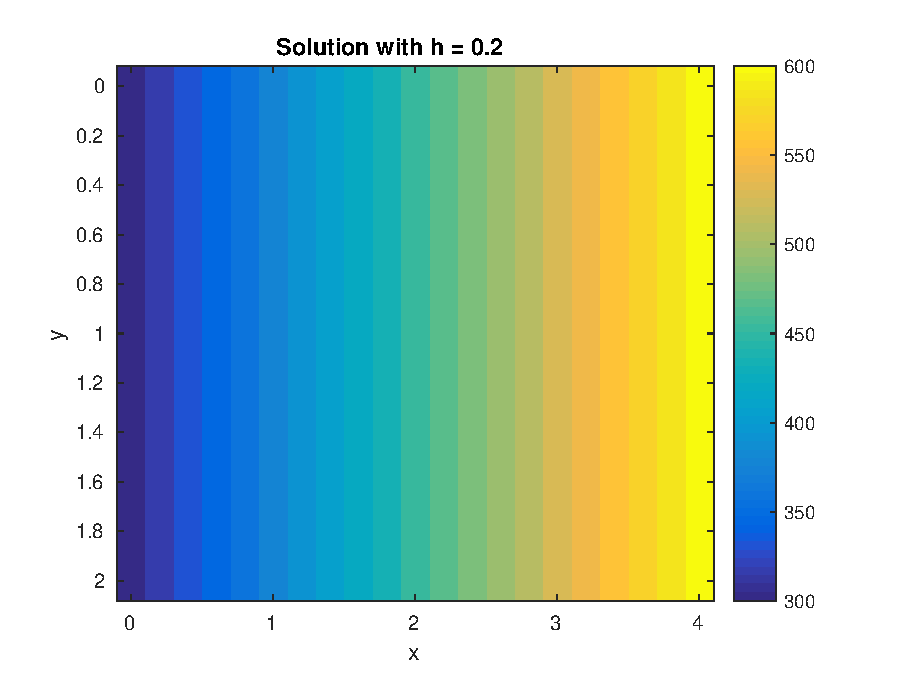
\includegraphics[width = 0.7\textwidth]{./h02.eps}
\caption{Solution with matlab for $h = 0.2$}
\label{fig:h02}
\end{figure}

\begin{figure}[!h]
\centering
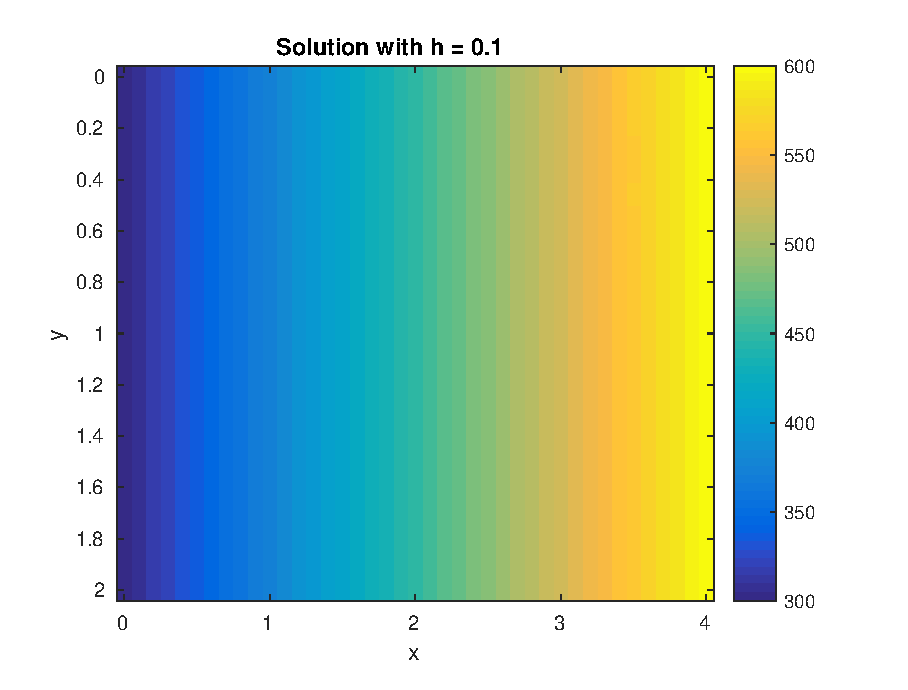
\includegraphics[width = 0.7\textwidth]{./h01.eps}
\caption{Solution with matlab for $h = 0.1$}
\label{fig:h01}
\end{figure}

\FloatBarrier

We see that the exact value at $(2,1)$ is close to $450$. It is clear by symmetry that the solution does not depend en the y-coordinate. Therefore the equation reduces to $$\dfrac{\dr^{2} T}{\dr x^{2}}=0.$$
The solution is a plane $$T(x,y)=T(x)= ax+b.$$ 
The boundary conditions $T(x=0)=300$ and $T(x=4)=600$ allow to find that $T(x)= 300+ 75x$. The solution respects boundary conditions~\eqref{eq:cond1} and~\eqref{eq:cond2}. It is now clear that $T(2,1)=450$. The (notably small) errors in the numerical solution are \textit{only} due to floating point computation errors. 

 
\section{Comsol Multiphysics solution}

In this section, we are going to solve the problem presented above with Comsol Multiphysics.

This is a Laplace equation and Comsol has already a nice setup for us. All we have to do is impose boundary conditions and generate the mesh. By default, Comsol sets zero flux boundary conditions so we just have to specify the Dirichlet conditions on the left and right sides. Once we have done this, we first use a mesh of type "normal". Figure \ref{mesh} shows what the "normal" mesh looks like for our geometry.

This mesh contains 316 triangles and 679 degrees of freedom. There are also 182 nodes.

\begin{figure}
\begin{center}
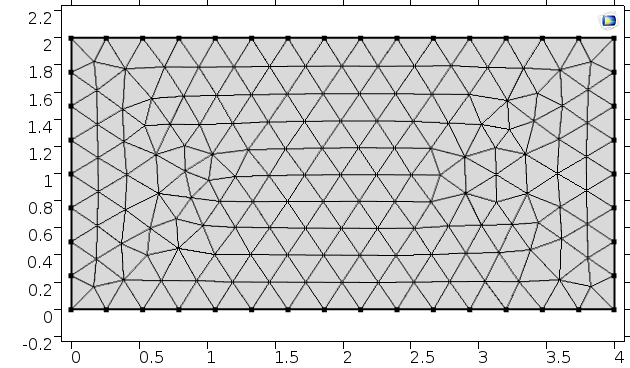
\includegraphics[scale=0.6]{laplaceMesh.png}
\caption{"Normal" mesh for the rectangular geometry}
\label{mesh}
\end{center}
\end{figure}

Figure \ref{rect} shows the solution for this choice of mesh. We can see that is it very similar to the one in section 1 which is a linear function between $x=0$ and $x=4$. We also used a probe to check the temperature at $(x,y)=(2,1)$.
$$T(2,1) = 450.0000000001594$$

That is very close to the analytic value and the error is only due to floating point computation.

We are now going to refine the mesh. We switch from "normal" to "fine". There are now 476 triangles and 1011 degrees of freedom, as well as 268 nodes.

We have another $T-value$ and:
$$T(2,1) = 450.000000000236$$

We can see that the two values are extremely close to each other and as we said, the small difference is due to floating point errors.

We finally restart all over again with a "normal" mesh. After having set all needed values, Comsol plots the solution given in figure \ref{rect}.


\begin{figure}
\begin{center}
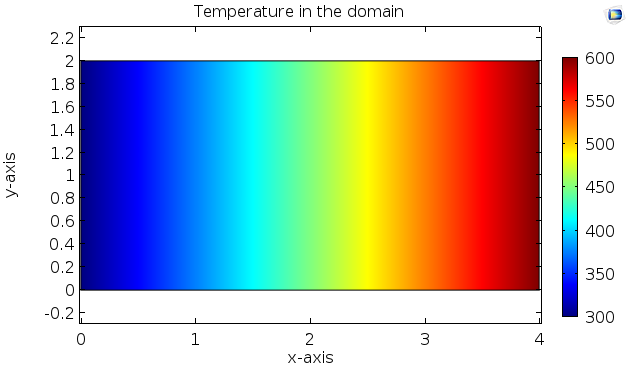
\includegraphics[scale=0.6]{laplaceRect.png}
\caption{Solution of the given problem with Comsol}
\label{rect}
\end{center}
\end{figure}

\section{More Comsol}

blu 

\section*{Codes}
\lstinputlisting{laplace.m}

\end{document}